\documentclass[tikz]{standalone}

\begin{document}

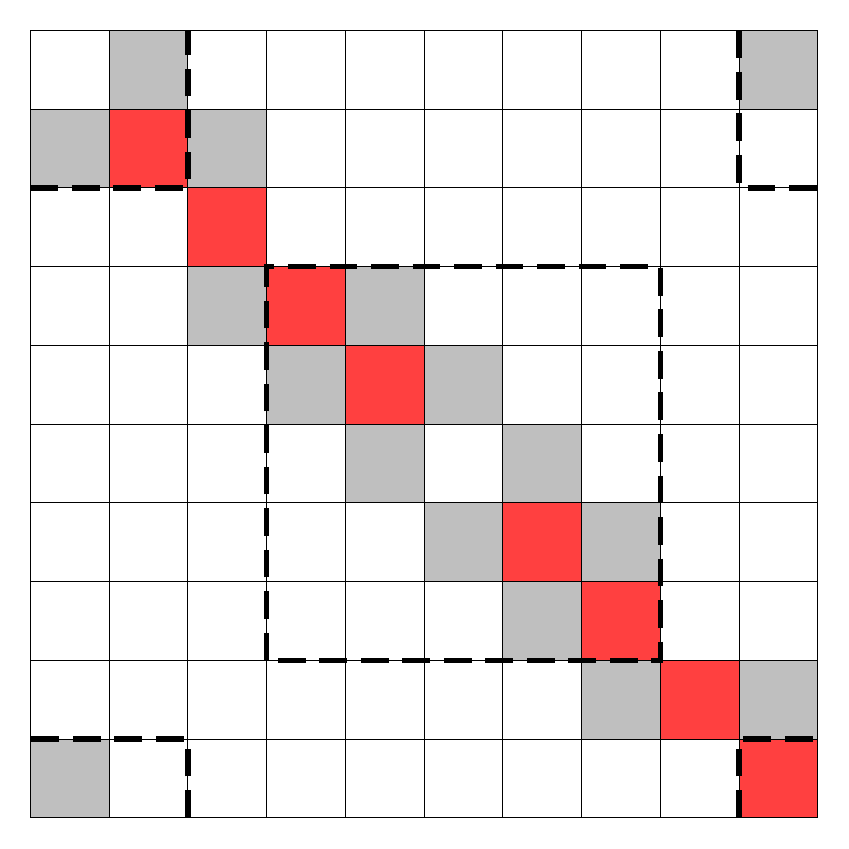
\begin{tikzpicture}

% 棋盘大小
\def\boardSize{9}

% 绘制棋盘
\foreach \x in {0,...,\boardSize} {
    \foreach \y in {0,...,\boardSize} {
        % 默认格子颜色为白色
        \fill[white] (\x, \y) rectangle (\x+1, \y+1);
        % 染成黑色的格子
        \ifnum\x=0 \ifnum\y=8 \fill[gray!50] (\x, \y) rectangle (\x+1, \y+1); \fi \fi
        %\ifnum\x=1 \ifnum\y=7 \fill[gray!50] (\x, \y) rectangle %(\x+1, \y+1); \fi \fi
        \ifnum\x=2 \ifnum\y=6 \fill[gray!50] (\x, \y) rectangle (\x+1, \y+1); \fi \fi
        \ifnum\x=3 \ifnum\y=5 \fill[gray!50] (\x, \y) rectangle (\x+1, \y+1); \fi \fi
        \ifnum\x=4 \ifnum\y=4 \fill[gray!50] (\x, \y) rectangle (\x+1, \y+1); \fi \fi
        \ifnum\x=5 \ifnum\y=3 \fill[gray!50] (\x, \y) rectangle (\x+1, \y+1); \fi \fi
        \ifnum\x=6 \ifnum\y=2 \fill[gray!50] (\x, \y) rectangle (\x+1, \y+1); \fi \fi
        \ifnum\x=7 \ifnum\y=1 \fill[gray!50] (\x, \y) rectangle (\x+1, \y+1); \fi \fi
         %\ifnum\x=8 \ifnum\y=0 \fill[gray!50] (\x, \y) rectangle %(\x+1, \y+1); \fi \fi
        

        \ifnum\x=1 \ifnum\y=9 \fill[gray!50] (\x, \y) rectangle (\x+1, \y+1); \fi \fi
        \ifnum\x=2 \ifnum\y=8 \fill[gray!50] (\x, \y) rectangle (\x+1, \y+1); \fi \fi
        %\ifnum\x=3 \ifnum\y=7 \fill[gray!50] (\x, \y) rectangle %(\x+1, \y+1); \fi \fi
        \ifnum\x=4 \ifnum\y=6 \fill[gray!50] (\x, \y) rectangle (\x+1, \y+1); \fi \fi
        \ifnum\x=5 \ifnum\y=5 \fill[gray!50] (\x, \y) rectangle (\x+1, \y+1); \fi \fi
        \ifnum\x=6 \ifnum\y=4 \fill[gray!50] (\x, \y) rectangle (\x+1, \y+1); \fi \fi
        \ifnum\x=7 \ifnum\y=3 \fill[gray!50] (\x, \y) rectangle (\x+1, \y+1); \fi \fi
       % \ifnum\x=8 \ifnum\y=2 \fill[gray!50] (\x, \y) rectangle %(\x+1, \y+1); \fi \fi
        \ifnum\x=9 \ifnum\y=1 \fill[gray!50] (\x, \y) rectangle (\x+1, \y+1); \fi \fi
        \ifnum\x=10 \ifnum\y=0 \fill[gray!50] (\x, \y) rectangle (\x+1, \y+1); \fi \fi

        \ifnum\x=0 \ifnum\y=0 \fill[gray!50] (\x, \y) rectangle (\x+1, \y+1); \fi \fi
        \ifnum\x=9 \ifnum\y=9 \fill[gray!50] (\x, \y) rectangle (\x+1, \y+1); \fi \fi
        
        % 染成红色的格子

        \ifnum\x=1 \ifnum\y=8 \fill[red!75] (\x, \y) rectangle (\x+1, \y+1); \fi \fi

        \ifnum\x=2 \ifnum\y=7 \fill[red!75] (\x, \y) rectangle (\x+1, \y+1); \fi \fi

        \ifnum\x=3 \ifnum\y=6 \fill[red!75] (\x, \y) rectangle (\x+1, \y+1); \fi \fi

        \ifnum\x=4 \ifnum\y=5 \fill[red!75] (\x, \y) rectangle (\x+1, \y+1); \fi \fi

        \ifnum\x=6 \ifnum\y=3 \fill[red!75] (\x, \y) rectangle (\x+1, \y+1); \fi \fi

        \ifnum\x=7 \ifnum\y=2 \fill[red!75] (\x, \y) rectangle (\x+1, \y+1); \fi \fi

        \ifnum\x=8 \ifnum\y=1 \fill[red!75] (\x, \y) rectangle (\x+1, \y+1); \fi \fi

        \ifnum\x=9 \ifnum\y=0 \fill[red!75] (\x, \y) rectangle (\x+1, \y+1); \fi \fi
        
        % 绘制格子边框
        \draw (\x, \y) rectangle (\x+1, \y+1);

        
    }
}

\draw[dash pattern=on 10pt off 5pt, line width = 2pt] (3,2) rectangle (8,7);

\draw[dash pattern=on 10pt off 5pt, line width = 2pt] (2,0) to (2,1) to (0,1);

\draw[dash pattern=on 10pt off 5pt, line width = 2pt] (0,8) to (2,8) to (2,10);

\draw[dash pattern=on 10pt off 5pt, line width = 2pt] (9,0) to (9,1) to (10,1);

\draw[dash pattern=on 10pt off 5pt, line width = 2pt] (9,10) to (9,8) to (10,8);

\end{tikzpicture}

\end{document}